\documentclass{standalone}
\usepackage{tikz}
\usetikzlibrary{patterns, positioning}


\begin{document}
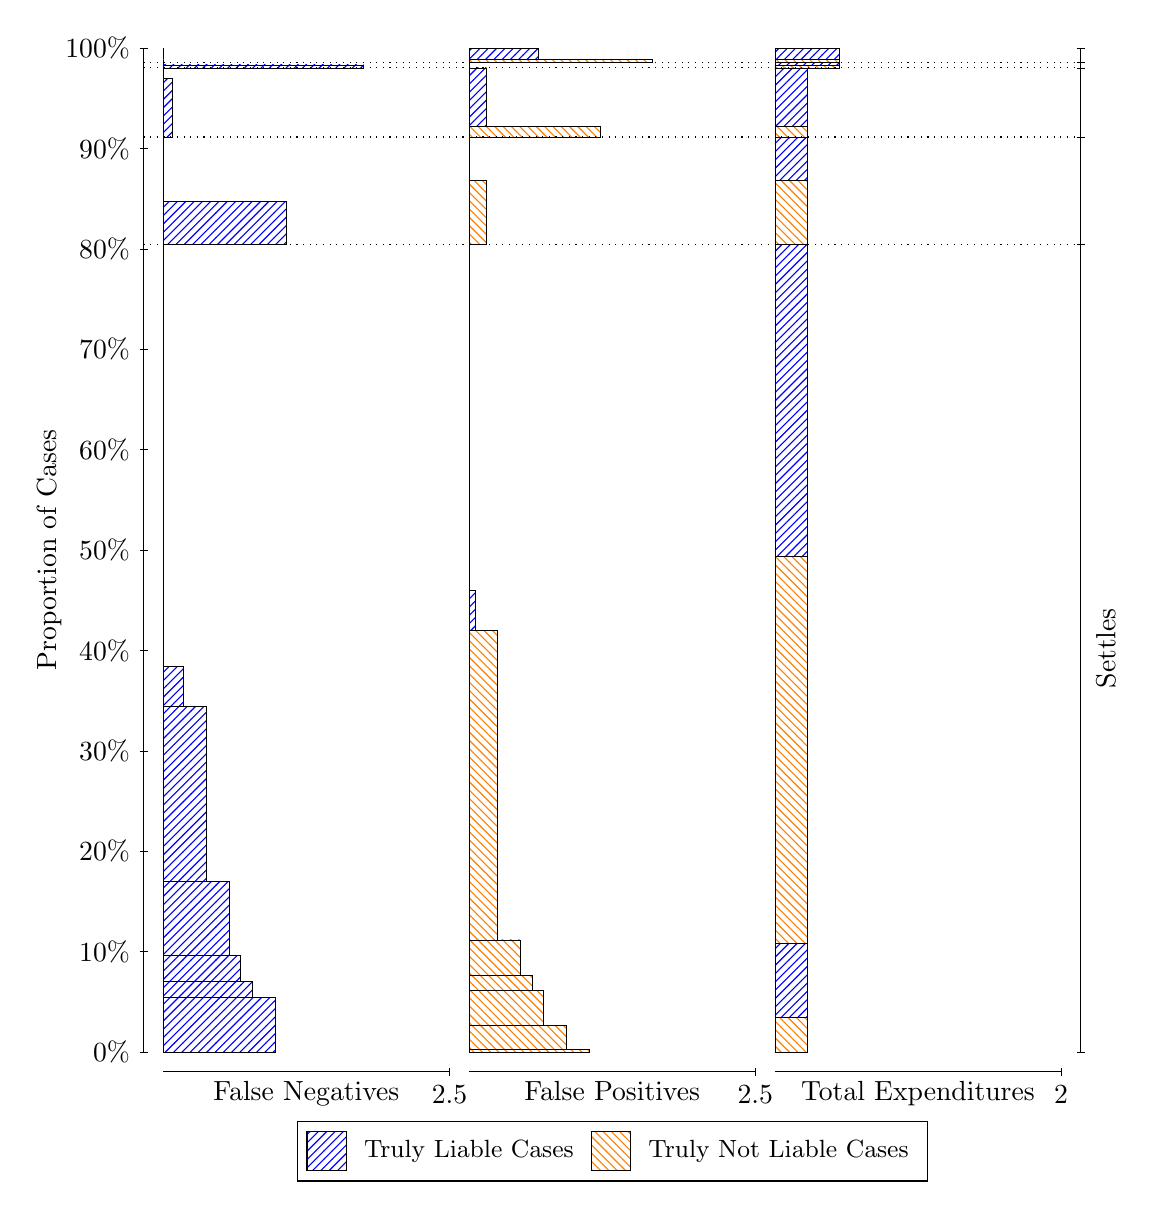
\begin{tikzpicture}
\draw[black, very thin] (1.5,1.75) -- (1.5,14.5);
\node[rotate=90, text=black, anchor=center] at (0.3, 8.125) {Proportion of Cases};
\draw[black, very thin] (1.45,1.75) -- (1.55,1.75);
\node[text=black, anchor=east] at (1.45, 1.75) {0\%};
\draw[black, very thin] (1.45,3.025) -- (1.55,3.025);
\node[text=black, anchor=east] at (1.45, 3.025) {10\%};
\draw[black, very thin] (1.45,4.3) -- (1.55,4.3);
\node[text=black, anchor=east] at (1.45, 4.3) {20\%};
\draw[black, very thin] (1.45,5.575) -- (1.55,5.575);
\node[text=black, anchor=east] at (1.45, 5.575) {30\%};
\draw[black, very thin] (1.45,6.85) -- (1.55,6.85);
\node[text=black, anchor=east] at (1.45, 6.85) {40\%};
\draw[black, very thin] (1.45,8.125) -- (1.55,8.125);
\node[text=black, anchor=east] at (1.45, 8.125) {50\%};
\draw[black, very thin] (1.45,9.4) -- (1.55,9.4);
\node[text=black, anchor=east] at (1.45, 9.4) {60\%};
\draw[black, very thin] (1.45,10.675) -- (1.55,10.675);
\node[text=black, anchor=east] at (1.45, 10.675) {70\%};
\draw[black, very thin] (1.45,11.95) -- (1.55,11.95);
\node[text=black, anchor=east] at (1.45, 11.95) {80\%};
\draw[black, very thin] (1.45,13.225) -- (1.55,13.225);
\node[text=black, anchor=east] at (1.45, 13.225) {90\%};
\draw[black, very thin] (1.45,14.5) -- (1.55,14.5);
\node[text=black, anchor=east] at (1.45, 14.5) {100\%};

\draw[black, very thin] (13.4,1.75) -- (13.4,14.5);
\draw[black, very thin] (13.35,1.75) -- (13.45,1.75);
\node[anchor=west] at (13.35, 1.75) {};
\draw[black, very thin] (13.35,12.005) -- (13.45,12.005);
\node[anchor=west] at (13.35, 12.005) {};
\draw[black, very thin] (13.35,13.37) -- (13.45,13.37);
\node[anchor=west] at (13.35, 13.37) {};
\draw[black, very thin] (13.35,14.249) -- (13.45,14.249);
\node[anchor=west] at (13.35, 14.249) {};
\draw[black, very thin] (13.35,14.32) -- (13.45,14.32);
\node[anchor=west] at (13.35, 14.32) {};
\draw[black, very thin] (13.35,14.5) -- (13.45,14.5);
\node[anchor=west] at (13.35, 14.5) {};

\draw[black, very thin, pattern color=blue, pattern=north east lines] (1.75,1.75) rectangle (3.167,2.4397);
\draw[black, very thin, pattern color=blue, pattern=north east lines] (1.75,2.4397) rectangle (2.8763,2.6485);
\draw[black, very thin, pattern color=blue, pattern=north east lines] (1.75,2.6485) rectangle (2.731,2.9791);
\draw[black, very thin, pattern color=blue, pattern=north east lines] (1.75,2.9791) rectangle (2.5857,3.9206);
\draw[black, very thin, pattern color=blue, pattern=north east lines] (1.75,3.9206) rectangle (2.295,6.1417);
\draw[black, very thin, pattern color=blue, pattern=north east lines] (1.75,6.1417) rectangle (2.0043,6.6503);
\draw[black, very thin, pattern color=orange, pattern=north west lines] (1.75,6.6503) rectangle (1.75,12.005);
\draw[black, very thin, pattern color=blue, pattern=north east lines] (1.75,12.005) rectangle (3.3123,12.557);
\draw[black, very thin, pattern color=orange, pattern=north west lines] (1.75,12.557) rectangle (1.75,13.37);
\draw[black, very thin, pattern color=blue, pattern=north east lines] (1.75,13.37) rectangle (1.859,14.113);
\draw[black, very thin, pattern color=orange, pattern=north west lines] (1.75,14.113) rectangle (1.75,14.249);
\draw[black, very thin, pattern color=blue, pattern=north east lines] (1.75,14.249) rectangle (4.2933,14.285);
\draw[black, very thin, pattern color=orange, pattern=north west lines] (1.75,14.285) rectangle (1.75,14.32);
\draw[black, very thin, pattern color=orange, pattern=north west lines] (1.75,14.32) rectangle (1.75,14.356);
\draw[black, very thin, pattern color=blue, pattern=north east lines] (1.75,14.356) rectangle (1.75,14.5);
\draw[black, very thin, pattern color=orange, pattern=north west lines] (5.6333,1.75) rectangle (7.1593,1.7864);
\draw[black, very thin, pattern color=orange, pattern=north west lines] (5.6333,1.7864) rectangle (6.8687,2.0926);
\draw[black, very thin, pattern color=orange, pattern=north west lines] (5.6333,2.0926) rectangle (6.578,2.5273);
\draw[black, very thin, pattern color=orange, pattern=north west lines] (5.6333,2.5273) rectangle (6.4327,2.7209);
\draw[black, very thin, pattern color=orange, pattern=north west lines] (5.6333,2.7209) rectangle (6.2873,3.1744);
\draw[black, very thin, pattern color=orange, pattern=north west lines] (5.6333,3.1744) rectangle (5.9967,7.1043);
\draw[black, very thin, pattern color=blue, pattern=north east lines] (5.6333,7.1043) rectangle (5.706,7.613);
\draw[black, very thin, pattern color=blue, pattern=north east lines] (5.6333,7.613) rectangle (5.6333,12.005);
\draw[black, very thin, pattern color=orange, pattern=north west lines] (5.6333,12.005) rectangle (5.8513,12.818);
\draw[black, very thin, pattern color=blue, pattern=north east lines] (5.6333,12.818) rectangle (5.6333,13.37);
\draw[black, very thin, pattern color=orange, pattern=north west lines] (5.6333,13.37) rectangle (7.3047,13.507);
\draw[black, very thin, pattern color=blue, pattern=north east lines] (5.6333,13.507) rectangle (5.8513,14.249);
\draw[black, very thin, pattern color=orange, pattern=north west lines] (5.6333,14.249) rectangle (5.6333,14.284);
\draw[black, very thin, pattern color=blue, pattern=north east lines] (5.6333,14.284) rectangle (5.6333,14.32);
\draw[black, very thin, pattern color=orange, pattern=north west lines] (5.6333,14.32) rectangle (7.9587,14.356);
\draw[black, very thin, pattern color=blue, pattern=north east lines] (5.6333,14.356) rectangle (6.5053,14.5);
\draw[black, very thin, pattern color=orange, pattern=north west lines] (9.5167,1.75) rectangle (9.9254,2.1847);
\draw[black, very thin, pattern color=blue, pattern=north east lines] (9.5167,2.1847) rectangle (9.9254,3.1262);
\draw[black, very thin, pattern color=orange, pattern=north west lines] (9.5167,3.1262) rectangle (9.9254,8.0458);
\draw[black, very thin, pattern color=blue, pattern=north east lines] (9.5167,8.0458) rectangle (9.9254,12.005);
\draw[black, very thin, pattern color=orange, pattern=north west lines] (9.5167,12.005) rectangle (9.9254,12.818);
\draw[black, very thin, pattern color=blue, pattern=north east lines] (9.5167,12.818) rectangle (9.9254,13.37);
\draw[black, very thin, pattern color=orange, pattern=north west lines] (9.5167,13.37) rectangle (9.9254,13.507);
\draw[black, very thin, pattern color=blue, pattern=north east lines] (9.5167,13.507) rectangle (9.9254,14.249);
\draw[black, very thin, pattern color=orange, pattern=north west lines] (9.5167,14.249) rectangle (10.334,14.284);
\draw[black, very thin, pattern color=blue, pattern=north east lines] (9.5167,14.284) rectangle (10.334,14.32);
\draw[black, very thin, pattern color=orange, pattern=north west lines] (9.5167,14.32) rectangle (10.334,14.356);
\draw[black, very thin, pattern color=blue, pattern=north east lines] (9.5167,14.356) rectangle (10.334,14.5);
\draw[black, dotted] (1.5,12.005) -- (13.4,12.005);
\draw[black, dotted] (1.5,13.37) -- (13.4,13.37);
\draw[black, dotted] (1.5,14.249) -- (13.4,14.249);
\draw[black, dotted] (1.5,14.32) -- (13.4,14.32);
\draw[black, very thin] (1.75,1.5) -- (5.3833,1.5);
\node[text=black, anchor=north] at (3.5667, 1.5) {False Negatives};
\draw[black, very thin] (5.3833,1.45) -- (5.3833,1.55);
\node[text=black, anchor=north] at (5.3833, 1.45) {2.5};

\draw[black, very thin] (5.6333,1.5) -- (9.2667,1.5);
\node[text=black, anchor=north] at (7.45, 1.5) {False Positives};
\draw[black, very thin] (9.2667,1.45) -- (9.2667,1.55);
\node[text=black, anchor=north] at (9.2667, 1.45) {2.5};

\draw[black, very thin] (9.5167,1.5) -- (13.15,1.5);
\node[text=black, anchor=north] at (11.333, 1.5) {Total Expenditures};
\draw[black, very thin] (13.15,1.45) -- (13.15,1.55);
\node[text=black, anchor=north] at (13.15, 1.45) {2};

\node[text=black, centered, rotate=90] at (13.72, 6.8773) {Settles};





\draw (7.449999999999999,1.5) node[draw=none] (baseCoordinate) {};
\begin{scope}[align=center]
        \matrix[scale=0.5, draw=black, below=0.5cm of baseCoordinate, nodes={draw}, column sep=0.1cm]{
            \node[rectangle, draw, minimum width=0.5cm, minimum height=0.5cm, pattern color=blue, pattern=north east lines] {}; &
            \node[draw=none, font=\small, text=black] (B) {Truly Liable Cases}; &
            \node[rectangle, draw, minimum width=0.5cm, minimum height=0.5cm, pattern color=orange, pattern=north west lines] {}; &
            \node[draw=none, font=\small, text=black] (B) {Truly Not Liable Cases}; \\
            };
\end{scope}

\end{tikzpicture}
\end{document}